
\chapter{Discrete control elements}

The word ``discrete'' means \textit{individual} or \textit{distinct}.  In engineering, a ``discrete'' variable or measurement refers to a true-or-false condition.  Thus, a discrete control element is one that has but a limited number of states (usually two: on and off).  In the case of valves, this means a valve designed to operate either in ``open'' mode or ``closed'' mode, not in-between.  \index{Discrete}





\filbreak
\section{On/off valves}

An on/off valve is the fluid equivalent of an electrical switch: a device that either allows unimpeded flow or acts to prevent flow altogether.  These valves are often used for routing process fluid to different locations, starting and stopping batch processes, and engaging automated safety (shutdown) functions.

Valve styles commonly used for on/off service include ball, plug, butterfly (or disk), gate, and globe.  Large on/off valves are generally of such a design that the full-open position provides a nearly unimpeded path for fluid to travel through.  Ball, plug\footnote{A \textit{plug} valve is very much like a ball valve, the difference being the shape of the rotating element.  Rather than a spherical ball, the plug valve uses a truncated cone as the rotary element, a slot cut through the cone serving as the passageway for fluid.  The conical shape of a plug valve's rotating element allows it to wedge tightly into the ``closed'' (shut) position for exceptional sealing.}, and gate valves provide just this characteristic:

$$\includegraphics{valve_54.eps}$$ \index{Ball valve} \index{Butterfly valve} \index{Disk valve} \index{Gate valve} \index{Diaphragm valve}

\filbreak

A series of photographs showing a cut-away ball valve (hand-actuated) in three different positions reveals the inner workings common to all ball valve mechanisms:

$$\includegraphics[width=1.75in]{valve_104.eps} \hskip 10pt \includegraphics[width=1.75in]{valve_105.eps} \hskip 10pt \includegraphics[width=1.75in]{valve_106.eps}$$

The left-hand image shows the valve in the shut position, with the bore axis facing the viewer (preventing fluid flow).  The right-hand image shows the valve in the open position, with the bore axis perpendicular to view and allowing flow.  The middle image shows the valve in a partially-open condition.

% ADD: Chopper valves as examples of on/off valves, used for safety shutdown systems
% ADD: ``Clay'' valves as examples of pilot-actuated valves











\filbreak
\section{Fluid power systems}

\label{Fluid power systems}

Given the ability of pressurized fluids to transmit force over long distances, it is not surprising that many practical ``fluid power systems'' have been built using fluid as a mechanical power-conducting media.  Fluid systems may be broadly grouped into \textit{pneumatic} (\underbar{gas}, usually air) and \textit{hydraulic} (\underbar{liquid}, usually oil\footnote{While it would be technically possible to use water instead of oil in a hydraulic power system, oil enjoys some distinct advantages.  First, oil is a lubricating substance, and non-corrosive, unlike water.  Second, oil enjoys a wider operating temperature range than water, which tends to both freeze and boil more readily.}).

Although there is no particular reason why a fluid power system must be discrete and not continuous, the majority of fluid power systems operate in an on/off control mode rather than throttling, which is why this subject is covered in the ``Discrete Control Elements'' chapter.

As usual for technical specialties, fluid power has its own unique symbology for describing various components and their interconnections.  The following diagram shows some common symbols used in fluid power system diagrams.  Lines connecting components together in a fluid power diagram indicate pipes, hoses, or tubes, much like lines connecting components together in an electronic schematic diagram represent wires:

$$\includegraphics{fluids_13.eps}$$

\vskip 10pt

\filbreak

Many of these symbols are self-explanatory, especially the pumps, motors, and cylinders.  What seems to cause the most confusion for people new to this symbology are the spool valve symbols.  A ``spool'' valve is a special type of flow-directing valve used in pneumatic and hydraulic systems to direct the pressurized fluid to different locations.  The symbology for a spool valve is a set of boxes, each box containing arrows or other symbols showing the intended direction(s) for the fluid's travel.  Take for instance this pneumatic reversing cylinder control system:

$$\includegraphics{fluids_14.eps}$$

The proper way to interpret a spool valve symbol is to see only one ``box'' active at any given time.  As the actuator (in this case, a hand-actuated lever) is moved one way or the other, the boxes ``shift'' laterally to redirect the flow of fluid from source to load.

\filbreak

For example, when the spool valve in this reversing control system is in its center position, the outer boxes in the symbol are inactive.  This is emphasized in the following diagram by coloring the outer boxes grey.  In this position, the spool valve neither admits compressed air to the cylinder nor vents any air from the cylinder.  As a result, the piston within the cylinder holds its position:

$$\includegraphics{fluids_15.eps}$$

\filbreak

If the spool valve is actuated in one direction, the spool piece inside the valve assembly shifts, directing compressed air to one side of the cylinder while venting air from the other side.  This is shown in the following diagram by shifting the boxes to one side, lining up the ``active'' box with the cylinder and air supply/vent connections:

$$\includegraphics{fluids_16.eps}$$

\filbreak

If the spool valve is actuated in the other direction, the spool piece inside the valve assembly shifts again, switching the directions of air flow to and from the cylinder.  Compressed air still flows from the supply to the vent, but the direction within the cylinder is reversed.  This causes the piston to reverse its mechanical travel:

$$\includegraphics{fluids_17.eps}$$

Note that the boxes in a spool valve symbol are never shifted or grayed-out in color like this to represent the valve's state in a real fluid power diagram.  The previous illustrations were drawn this way only as an aid to your understanding, teaching you how to interpret the meaning of the symbols when you see them in real fluid power diagrams.  Like electrical switches represented in schematic diagrams, spool valve symbols are always drawn with the boxes aligned in their ``resting'' states, and with all portions identically colored.

\filbreak

Hydraulic systems require more components, including filters and pressure regulators, to ensure proper operation.  Shown here is a simple uni-directional hydraulic motor control system:

$$\includegraphics{fluids_18.eps}$$

Note the placement of the pressure relief valve: it is a \textit{shunt} regulator, bleeding excess pressure from the discharge of the hydraulic pump back to the reservoir\footnote{Note also how identical reservoir symbols may be placed at different locations of the diagram although they represent the exact same reservoir.  This is analogous to ``ground'' symbols in electronic schematic diagrams, every ground symbol representing a common connection to the same zero-potential point.}.  A ``shunt'' regulator is necessary because hydraulic pumps are \textit{positive displacement}, meaning they discharge a fixed volume of fluid with every revolution of the shaft.  If the discharge of a positive-displacement pump is blocked (as it would be if the spool valve were placed in its default ``off'' position, with no shunt regulator to bleed pressure back to the reservoir), it will mechanically ``lock'' and refuse to turn.  This would overload the electric motor coupled to the pump, if not for the pressure regulating valve providing an alternative route for oil to flow back to the reservoir.  This shunt regulator allows the pump to discharge a fixed rate of oil flow (for a constant electric motor speed) under all hydraulic operating conditions.  \index{Positive displacement pump}

\filbreak

An alternative to using a shunt regulating valve in a hydraulic system is to use a \textit{variable-displacement pump}.  Variable-displacement pumps still output a certain volume of hydraulic oil per shaft revolution, but that volumetric quantity may be varied by moving a component within the pump.  In other words, the pump's per-revolution displacement of oil may be externally adjusted.  \index{Variable displacement pump}

If we connect the variable-displacement mechanism of such a hydraulic pump to a pressure-sensing element such as a bellows, in a way where the pump senses its own discharge pressure and adjusts its volumetric output accordingly, we will have a pressure-regulating hydraulic system that not only prevents the pump from ``locking'' when the spool valve turns off, but also saves energy by not circulating pressurized oil all the time:

$$\includegraphics{fluids_19.eps}$$

Note the placement of a filter at the inlet of the pump in all hydraulic systems.  Filtration is an absolute essential for any hydraulic system, given the extremely tight dimensional tolerances of components inside pumps, motors, spool valves, and cylinders.  Even very small concentrations of particulate impurities in the hydraulic fluid may drastically shorten the life of these precision-machined components.

Hydraulic fluid also acts as a heat-transfer medium, and as such must be kept cool enough to prevent thermal damage to components.  Large hydraulic systems are equipped with coolers, which are just heat exchangers designed to extract heat energy from the fluid and transfer it to either cooling water or ambient air.  Small hydraulic systems dissipate heat at a fast enough rate through their components that coolers are often unnecessary.

\filbreak

An interior view of a simple ``2-way'' spool valve such as that used in the hydraulic motor system previously examined reveals why cleanliness and temperature stability is important.  The spool valve is shown here in both positions, with its accompanying schematic symbol:  \index{Spool valve illustration, 2-way}

$$\includegraphics{fluids_27.eps}$$

Both the spool and the valve body it moves in are circular in cross-section.  The spool has wide areas called ``lands'' that act to cover and uncover ports in the valve body for fluid to flow through.  The precise fit between the outside diameter of the lands and the inside diameter of the valve body's bore is the only factor limiting leakage through this spool valve in the closed state.  Dirty hydraulic fluid will wear at this precise fit over time until the valve is no longer capable of sealing fluid in its ``closed'' position.  Extreme cycles in temperature will also compromise the precise fit between the spool and the valve body.

Pneumatic fluid power systems require cleanliness as well, since any particulate contamination in the air will likewise cause undue wear in the close-tolerance compressors, motors, valves, and cylinders.  Unlike hydraulic oil, compressed air is not a natural lubricant, which means many pneumatic power devices benefit from a small concentration of oil vapor in the air.  Pneumatic ``oilers'' designed to introduce lubricating oil into a flowing air stream are generally located very near the point of use (e.g. the motor or the cylinder) to ensure the oil does not condense and ``settle'' in the air piping.

\vskip 10pt

\filbreak

Fluid power systems in general tend to be inefficient, requiring much more energy input to the fluid than what is extracted at the points of use\footnote{Close-coupled hydraulic systems with variable-displacement pumps and/or motors may achieve high efficiency, but they are the exception rather than the rule.  One such system I have seen was used to couple a diesel engine to the drive axle of a large commercial truck, using a variable-displacement pump as a continuously-variable transmission to keep the diesel engine in its optimum speed range.  The system was so efficient, it did not require a cooler for the hydraulic oil!}.  When large amounts of energy need to be transmitted over long distances, electricity is the a more practical medium for the task.  However, fluid power systems enjoy certain advantages over electric power, a few of which are listed here:

\begin{itemize}
\item Fluid power motors and cylinders do not overload at low speeds or under locked conditions
\item Fluid power systems present little hazard of accidently igniting flammable atmospheres (i.e. no sparks produced)
\item Fluid power systems present little or no fire hazard\footnote{Many kinds of hydraulic oils are flammable, so this is not a perfectly true statement.  However, fire-resistant fluids such as \textit{Skydrol} (introduced to the aviation industry for safety) are commercially available.} \index{Skydrol hydraulic fluid}
\item Fluid power systems present no hazard of electric shock or arc flash
\item Fluid power systems are often easier to understand and troubleshoot than electric systems
\item Fluid power systems may be safely used in submerged (underwater) environments
\item Pneumatic systems are relatively easy to equip with back-up energy reserve (e.g. liquefied nitrogen serving as a back-up gas supply in the event of compressor shut-down)
\item Pneumatic systems are self-purging (i.e. enclosures housing pneumatic devices will be naturally purged of dusts and vapors by leaking air)
\end{itemize}

\vskip 10pt

Another important consideration for fluid power systems is the ongoing maintenance work they require for reliable operation.  Hydraulic power systems will suffer rapid wear if the hydraulic oil is not clean and chemically stable.  The fluid in a hydraulic system not only transmits mechanical power, but it also lubricates and stabilizes the temperature of components as they transfer that power between different forms.  Regular filter changes and oil changes (especially if the fluid is subject to contamination from the process) is necessary for long service life of any hydraulic system.  

Pneumatic (instrument air) systems must be free of water vapor and particulate contamination for much the same reason.  Water is perhaps the most common contaminant in instrument air systems, causing corrosion of metal components and subsequent clogging of orifices.  Special devices called \textit{air dryers} installed in instrument air systems use solid materials called \textit{desiccants} to absorb water entrained in the compressed air.  The desiccant material is ``regenerated'' by the dryer mechanism on a regular cycle, but must be periodically replaced when its water-absorbing ability wanes.  \index{Dryer, instrument air}  \index{Air dryer}  \index{Desiccant}

\filbreak

This next photograph shows a high-capacity industrial air dryer, with two large chambers holding desiccant:

$$\includegraphics[width=5in]{fluids_25.eps}$$

A valving system directs the main flow of compressed air through one of these desiccant chambers at a time, allowing the desiccant to absorb water vapor in the air.  Meanwhile, the unused chamber is purged of its collected water by venting low-pressure air through it to the atmosphere.  An electronic timer unit (or PLC) controls the cycling of this valve system to ensure adequate drying and maximized desiccant service life.

Moisture content in instrument air is often expressed by the term \textit{dew point}.  This is the temperature at which water vapor suspended in the instrument air will condense into water droplets, at atmospheric pressure.  The ``drier'' the air, the lower the dew point temperature; the ``wetter'' the air, the higher the dew point temperature.  Sometimes the ``dryness'' of instrument air is expressed in terms of \textit{pressure dew point} (PDP), which is the temperature of water condensation at system pressure rather than at atmospheric pressure.  Pressure dew point is always a higher temperature value than atmospheric dew point, since greater air pressures force condensation to occur more readily.  Pressure dew point is a more practical value than atmospheric dew point for an instrument air system, as PDP directly indicates the ambient temperature at which water will condense in an \textit{operating} pneumatic system.  A low dew point value means that the air dryer is working as it should.  A high dew point value means condensation is more likely to form in the compressed air system piping.  \index{Dew point}

\filbreak

A simple way to help extract water from an instrument air system is an accessory called a \textit{water trap}, usually found on air pressure regulators.  The following photograph shows a Fisher pneumatic regulator equipped with such a trap on the bottom:

$$\includegraphics[height=3in]{fluids_26.eps}$$

A shiny metal ``wingnut'' drain appears at the very bottom of the regulator, acting as a manual valve for purging collected water from the basin where compressed air enters the regulator mechanism.  Periodic opening of this drain valve by maintenance or operations personnel allows collected water to be blown out of the regulator.

\vskip 10pt

\filbreak

Another way to help minimize the amount of water reaching pneumatic devices is to properly orient all connections to the main air pipe (called a \textit{header}).  Ideally, each instrument air tap coming off a header should do so on the \textit{top} of the header, not the bottom.  This way, collected condensation inside the header will not go directly to the points of use, but rather will drain downhill to the lowest point in the header where a drain valve may be placed.

This next photograph shows an \textit{incorrect} installation, where air is drawn off the bottom of the main header line:

$$\includegraphics[width=4in]{fluids_32.eps}$$

Such an installation invites trouble, as every bit of water condensed inside the header pipe is \textit{guaranteed} to find its way by gravity to the instruments connected to the underside of that header.

One good feature of this installation is the use of stainless steel as the piping material.  Copper, brass, plastic\footnote{Certain types of plastic pipe such as PVC should never be used in compressed air systems because it becomes brittle and liable to fracture over time.  If you are considering the use of plastic for a high-pressure compressed air system, be sure the type of plastic is engineered for air pressure service!}, and stainless steel are the preferred materials for instrument air piping, tubing, valves, and fittings, as standard (iron) pipe will inevitably rust in the presence of condensation.  Particles of rust created inside an instrument air system plays havoc with the tiny ports, nozzles, and orifices of pneumatic instruments.

\filbreak

The proper way to make instrument air connections to the air header is as such:

$$\includegraphics{fluids_33.eps}$$

In order to facilitate draining of the header, the header should be slightly inclined, with the drain valve installed at the lowest point.  This drain valve should then be periodically opened on a regular maintenance schedule in order to prevent the header from slowly filling up with condensed water over time.







\filbreak
\section{Solenoid valves}

A very common form of on/off valve used for pneumatic and hydraulic systems alike is the \textit{solenoid valve}.  A ``solenoid'' is nothing more than a coil of wire designed to produce a magnetic field when energized.  Solenoid actuators work by attracting a movable ferrous \textit{armature} into the center of the solenoid coil when energized, the force of this attraction working to actuate a small valve mechanism. \index{Solenoid valve}

Solenoid-actuated valves are usually classified according to the number of ports (``ways'').  A simple on/off solenoid valve controlling flow into one port and out of another port is called a \textit{2-way} valve.  Another style of solenoid valve, where flow is directed in one path or to another path -- much like a single-pole double-throw (SPDT) electrical switch -- is called a \textit{3-way} valve because it has three fluid ports.



\filbreak
\subsection{2-way solenoid valves}

2-way solenoid valves operate in a manner analogous to single-pole single-throw (SPST) electrical switches: with only one path for flow.

Solenoid valve symbols often appear identical to fluid power valve symbols, with ``boxes'' representing flow paths and directions between ports in each of the valve's states.  Like electrical switches, these valve symbols are always drawn in their ``normal'' (resting) state, where the return spring's action determines the valve position:  \index{Normal state of a valve}

$$\includegraphics{discrete15.eps}$$

% ADD: cutaway view of two-way spool-type valve mechanism

\filbreak

A good way to make sense of these ``box'' valve symbols is to imagine the boxes sliding back and forth as the actuating elements work.  For example, the two boxes in a normally-closed solenoid valve symbol may be thought of in terms of being \textit{pushed} to the left by the spring when de-energized and \textit{pushed} to the right by the solenoid's force when energized.  Here, the color grey de-emphasizes the unselected box in each of the valve's two states:

$$\includegraphics{discrete30.eps}$$

As with electrical switches in schematic diagrams, fluid control valve symbols are always drawn in their ``normal'' (resting) states.  For example, a normally-closed valve will always be drawn so that the box with the blocked ports aligns with the tubes leading to and from the valve.  What you see in the above illustration are ``dramatized'' symbols, highlighting the valve's action by color and by re-positioning the boxes, strictly for the purpose of making it easier for you to grasp the concept.  This sort of coloring and re-positioning is \textit{never} shown in a real schematic diagram.  In a fluid control schematic, it is left to the reader to visualize the valve symbol boxes moving to and fro, determining the flow path of fluid through the valve.

Unlike electrical switches, of course, the terms \textit{open} and \textit{closed} have opposite meanings for valves.  An ``open'' electrical switch constitutes a break in the circuit, ensuring no current; an ``open'' valve, by contrast, freely allows fluid flow through it.  A ``closed'' electrical switch has continuity, allowing current through it; a ``closed'' valve, on the other hand, shuts off fluid flow.

\filbreak

The arrow inside a solenoid valve symbol actually denotes a preferred direction of flow.  Most solenoid valves use a ``globe'' or ``poppet'' style of valve element, where a metal plug covers up a hole (called the ``seat'').  Process fluid pressure should be applied to the valve in such a way that the pressure difference tends to hold the solenoid valve in its ``normal'' position (the same position as driven by the return spring).  Otherwise\footnote{One could argue that enough fluid pressure could override the solenoid's energized state as well, so why choose to have the fluid pressure act in the direction of helping the return spring?  The answer to this (very good) question is that the solenoid's energized force greatly exceeds that of the return spring.  This is immediately obvious on first inspection, as the solenoid \textit{must} be stronger than the return spring or else the solenoid valve would never actuate!  Furthermore, the solenoid's force must be \textit{significantly} stronger than the spring, or else the valve would open rather slowly.  Fast valve action demands a solenoid force that greatly exceeds spring force.  Realizing this, now, we see that the spring is the weaker of the two forces, and thus it makes perfect sense why we should use the valve in such a way that the process pressure helps the spring: the solenoid's force has the best chance of overcoming the force on the plug produced by process pressure, so those two forces should be placed in opposition, while the return spring's force should work \textit{with} (not against) the process pressure.}, enough fluid pressure might override the return spring's action, preventing the valve from achieving its ``normal'' state when de-energized.  Thus, we see that the label ``2-way'' does not refer to two directions of flow as one might assume, but rather two \textit{ports} on the valve for fluid to travel through.

Some solenoid valves are designed in such a way that the direction of fluid flow through them is irrelevant.  In such valves, the arrow symbols will be double-headed (one head at each end, pointing in opposite directions) to show the possibility of flow in either direction.

$$\includegraphics{discrete31.eps}$$




\filbreak
\subsection{3-way solenoid valves}

3-way solenoid valves operate in a manner analogous to single-pole double-throw (SPDT) electrical switches: with two paths for flow sharing one common terminal.

3-way solenoid valves have three ports for fluid, and like 2-way valves may be referred to either as \textit{normally-open} and \textit{normally-closed}.  Ports on a pneumatic 3-way valve are commonly labeled with the letters ``P,'' ``E,'' and ``C,'' representing \textit{Pressure} (compressed air supply), \textit{Exhaust} (vent to atmosphere), and \textit{Cylinder} (the actuating mechanism), respectively.  Alternatively, you may see the cylinder port labeled ``A'' (for \textit{actuator}) instead of ``C''.  If the solenoid valve is intended for use in a hydraulic (liquid) system, the letter ``T'' is customarily used to identify the return port rather than ``E'' (i.e. \textit{Tank} rather than \textit{Exhaust}):

$$\includegraphics{discrete16.eps}$$

The letters used to label ports on a valve such as this not only denote those ports' destinations, but also serve to mark which ``box'' of the valve's symbol is the normal (resting) state.  In all fluid power diagrams you will see that only one of the boxes on each spool valve will have lines connecting to it and/or labels at the fluid ports, and that box is the one which will be aligned when the valve is not being actuated.  \index{Normal state of a valve}

\filbreak

Alternatively, the numbers 1, 2, and 3 may be used to label the same ports.  However, the numbers do not consistently refer to pressure source (P) and exhaust (E) ports, but rather to the 3-way valve's ``normal'' versus ``actuated'' statuses.  A 3-way valve will pass fluid between ports 1 and 3 in its ``normal'' (resting) state, and pass fluid between ports 1 and 2 in its energized state.  The following table shows the correspondence between port numbers and port letters for both styles of 3-way solenoid valve:

% No blank lines allowed between lines of an \halign structure!
% I use comments (%) instead, so that TeX doesn't choke.

$$\vbox{\offinterlineskip
\halign{\strut
\vrule \quad\hfil # \ \hfil & 
\vrule \quad\hfil # \ \hfil & 
\vrule \quad\hfil # \ \hfil & 
\vrule \quad\hfil # \ \hfil \vrule \cr
\noalign{\hrule}
%
% First row
\textbf{Valve type} & \textbf{Pressure port} (P) & \textbf{Exhaust port} (E) & \textbf{Cylinder port} (C) \cr
%
\noalign{\hrule}
%
% Another row
Normally-closed & 2 & 3 & 1 \cr
%
\noalign{\hrule}
%
% Another row
Normally-open & 3 & 2 & 1 \cr
%
\noalign{\hrule}
} % End of \halign 
}$$ % End of \vbox

Another way to think of this labeling is to consider port 1 the \textit{common}, port 2 the \textit{normally-closed}, and port 3 the \textit{normally-open}, in a manner similar to SPDT (form-C) electrical switches.  Again, bear in mind that the words ``open'' and ``closed'' do not mean the same for fluid valves as they do for electrical switches.  A ``normally-open'' port on the valve permits fluid flow in its ``normal'' state, whereas a ``normally-open'' switch contact \textit{prevents} electric current flow in its ``normal'' state.

As with 2-way solenoid valves, the arrows denote preferred direction of fluid flow.  Bidirectional 3-way valves will be drawn with double-headed arrows (pointing both directions).

\vskip 10pt

\filbreak

A different symbology is used in loop diagrams and P\&IDs than that found in fluid power diagrams -- one more resembling general instrumentation (ISA) valve symbols:

$$\includegraphics{discrete17.eps}$$

\filbreak

Regrettably, these symbols are not nearly as descriptive as those used in fluid power diagrams.  In order to show directions of flow (especially for 3-way valves), one must add arrows showing ``normal'' (resting, \textit{DE}) flow directions:

$$\includegraphics{discrete18.eps}$$

\filbreak

Alternatively, a \textit{pair} of arrows shows the directions of flow in both energized (\textit{E}) and de-energized (\textit{D}) states:

$$\includegraphics{discrete19.eps}$$

\filbreak

Photographs of an actual 3-way solenoid valve (this one manufactured by ASCO) appear here:  \index{ASCO solenoid valve}

$$\includegraphics[width=2.5in]{discrete24.eps} \hskip 30pt \includegraphics[width=2.5in]{discrete25.eps}$$

\filbreak

A view of the nameplate for this particular solenoid valve reveals some of its ratings and characteristics:

$$\includegraphics[width=4in]{discrete26.eps}$$




\filbreak
\subsection{4-way solenoid valves}

When a pneumatic actuator requires air pressure applied to two different ports in order to move two different directions (such as the case for cylinders lacking a return spring), the solenoid valve supplying air to that actuator must have four ports: one for air supply (P), one for exhaust (E), and two for the cylinder ports (typically labeled A and B).  The following diagram shows a 4-way solenoid valve connected to the piston actuator of a larger (process) ball valve:

$$\includegraphics{discrete22.eps}$$

\filbreak

The same diagram could be drawn using the ``triangle'' solenoid valve symbols rather than the ``block'' symbols more common to fluid power diagrams:

$$\includegraphics{discrete23.eps}$$

Here, the letters ``D'' and ``E'' specify which directions air is allowed to flow when the solenoid is de-energized and energized, respectively.

\vskip 10pt

In both of the examples shown above, the solenoid valve forces the piston-actuated valve stem to move down (shut off) when the solenoid is de-energized.  When the solenoid is energized, air is directed to the bottom of the piston (with the top of the piston becoming vented to atmosphere), causing the piston-actuated valve stem to move up (open wide).


\filbreak

An interior view of a standard spool-type 4-way valve of the kind commonly used for directional hydraulic\footnote{In hydraulics, it is common to use the letter ``T'' to represent the \textit{tank} or \textit{reservoir} return connection rather than the letter ``E'' for \textit{exhaust}, which is why the supply and vent lines on this valve are labeled ``P'' and ``T'', respectively.} controls is shown here, along with its accompanying schematic symbol:  \index{Spool valve illustration, 4-way}

$$\includegraphics{fluids_28.eps}$$

Note that the actuator (e.g. hand lever, solenoid armature, etc.) has been omitted from this illustration for simplicity.  Only the spool and valve body are shown.

\filbreak

A variation on this theme uses a shorter spool allowing the two control ports to freely pass fluid in the ``normal'' position:  \index{Spool valve illustration, 4-way}  \index{Normal state of a valve}

$$\includegraphics{fluids_30.eps}$$

Such a 4-way valve is useful for applications where the final control element (motor, cylinder) must be free to move rather than be locked in place with the valve in the middle position.

\filbreak

If no center ``off'' position is needed, the lands may be shortened in such a way that they cannot fully cover the ``P,'' ``1,'' and ``2'' ports simultaneously, making the valve useful only in its two extreme positions:  \index{Spool valve illustration, 4-way}

$$\includegraphics{fluids_29.eps}$$

Not all 4-way valves use the spool-type design.  However, the spool valve enjoys the advantage of having \textit{pressure balance} on its one moving part.  If you examine these cut-away illustrations closely, you will see that the two lands present equal surface areas to the two pressures (pump and tank, ``P'' and ``T'') in perfect vertical symmetry, such that any forces acting on the two lands from fluid pressure do so in opposite directions.  This means there will be no net hydraulic force acting on the spool to interfere with its positioning, thus making it very easy to position by hand lever, solenoid, piston, etc.

\filbreak

A photograph of a Parker brand 4-way pneumatic solenoid valve appears here:

$$\includegraphics[width=6in]{fluids_31.eps}$$

This particular solenoid valve is spring-centered, with one solenoid coil at each end to provide actuation in two different directions.  The middle position is one where all ports are blocked, providing a ``locked'' control position for the pneumatic actuating element fed air by this solenoid valve.










\filbreak
\subsection{Normal energization states}

Solenoid valves may be used in such a way that they spend most of their time de-energized, energizing only for brief periods of time when some special function is required.  Alternatively, solenoids may be maintained in an energized state, and de-energized to perform their design function.  The choice to use a solenoid's energized or de-energized state to perform a specific function is left to the system designer, but nevertheless it is important for all maintenance personnel to know in order to perform work on a solenoid-controlled system.

Take the following segment of an actual P\&ID for a steam turbine-driven pump control system for example, where a pair of 3-way solenoid valves control instrument air pressure\footnote{The letters ``IAS'' refer to \textit{instrument air supply}.} to a piston-actuated steam valve to start the turbine in the event that an electric motor-driven pump happens to fail:
qqqq pv
$$\includegraphics[width=5in]{discrete20.eps}$$

If \textit{either}\footnote{This solenoid valve arrangement would be designated \textit{1oo2} from the perspective of starting the turbine, since only one out of the two solenoids needs to trip in order to initiate the turbine start-up.} of the two solenoid valves de-energizes, instrument air pressure will vent from the top of the piston actuator to atmosphere, causing the steam valve to ``fail'' to the full-open position and send steam to the turbine.  This much is evident from the curved arrows showing air flowing to the ``Vent'' ports in a de-energized (DE) condition.  An additional valve (PY-590) guarantees the piston actuator's upward motion by simultaneously applying air pressure to the bottom\footnote{If you examine this diagram closely, you will notice an error in it: it shows the top and bottom of the piston actuator \textit{connected together} by air tubing, which if implemented in real life would prevent air pressure from imparting any force to the valve stem at all!  Connecting the top and bottom of the actuator together would ensure the piston always sees zero differential pressure, and thus would never develop a resultant force.  The output tube of PY-590 should only connect to the bottom of the piston actuator, not to the bottom \textit{and} the top.  A more minor error in this diagram snippet is the labeling of SOV-590A: it actually reads ``SOV-59DA'' if you look closely enough!  My first inclination when sampling this real P\&ID for inclusion in the book was to correct the errors, but I think an important lesson may be taught by leaving them in: documentation errors are a realistic challenge you will contend with on the job as an instrumentation professional!} of the actuator if ever air is vented from the top.  As an additional feature, the left-hand solenoid valve (SOV-590A) has a manual ``Reset'' lever on it, symbolized by the letter ``R'' inside a diamond outline.

The only indication of the solenoids' typical status (energized or de-energized) comes from the letters ``NE'' next to each solenoid coil.  In this case, ``NE'' stands for \textit{normally energized}.  Therefore, this steam turbine control system, which serves as a back-up to an electric motor-driven pump, relies on either (or both) of the solenoid valves \textit{de-energizing} to make the turbine start up.  Under ``normal'' conditions, where the turbine is not needed, the solenoids remain energized and the steam valve remains shut.  \index{Normally energized (NE)}  \index{NE}

\vskip 10pt

Unfortunately, this use of the word ``normal'' is altogether different from the use of the word ``normal'' when describing a solenoid valve's open/close characteristics.  Recall that a \textit{normally open} solenoid valve allows fluid to pass through when it is de-energized.  A \textit{normally closed} solenoid valve, by contrast, shuts off fluid flow when de-energized.  In this context, the word ``normally'' refers to the \textit{unpowered} state of the solenoid valve.  This is quite similar to how the word ``normally' is used to describe switch contact status: a normally-open (NO) electrical switch is open when unactuated (at rest); a normally-closed (NC) electrical switch is closed when unactuated (at rest).  In both cases, with solenoid valves and with electrical switches, the word ``normally'' refers to the resting condition of \textit{no stimulation}.   \index{Normal energization state of a solenoid} 

However, when an engineer designs a solenoid control system and declares a solenoid to be ``normally energized,'' that engineer is describing the \textit{typical} status of the solenoid valve \textit{as it is intended to function in the process}.  This may or may not correspond to the \textit{manufacturer's} definition of ``normally,'' since the solenoid manufacturer cannot possibly know which state any of their customers intends to have their solenoid valve typically operate in.  To illustrate using the previous steam turbine control system P\&ID, those two solenoid valves would be considered \textit{normally closed} by the manufacturer, since their de-energized states block air flow from the ``P'' port to the ``C'' port and vent air pressure from the ``C'' port to the ``E'' (vent) port.  However, the engineer who designed this system wanted both solenoids to be energized whenever the turbine was not needed to run (the ``normal'' state of the process), and so the engineer labeled both solenoid coils as \textit{normally energized}, which means both solenoids will be actuated to pass air pressure from their ``P'' ports to their ``C'' ports (and close off the vent ports) under typical conditions.  Here, we see the manufacturer's definition of ``normal'' for the solenoid valve body (i.e. the \textit{resting} condition) is precisely opposite that of the process engineer's definition of ``normal'' for the solenoid coil (i.e. the typical operating status of the process) in this particular application.

\filbreak

The manufacturer's and process engineer's definitions of ``normally'' are not always in conflict.  Take for example this P\&ID segment, showing the solenoid control of an air vent door on a large furnace, designed to open up if the forced-draft fan (blowing combustion air into the furnace) happens to stop for any reason:

$$\includegraphics[width=3.5in]{discrete21.eps}$$

Here we have a \textit{normally open} solenoid valve, designed by the manufacturer to pass instrument air pressure from the pressure (``P'') port to the cylinder (``C'') port when de-energized.  The straight arrow with the ``DE'' label next to it reveals this to be the case.  Instrument air pressure sent to the air door actuator holds the door shut, meaning the air door will swing open if ever instrument air pressure is vented by the solenoid.  For this particular solenoid, this would require an \textit{energized} condition.

The process engineer designing this Emergency Air Door control system chose to let the solenoid be in its de-energized state under typical operating conditions (when the furnace air door should be shut), a fact revealed by the letters ``NDE'' (normally de-energized) next to the solenoid coil symbol.  Therefore, the ``normal'' process operating condition for this solenoid happens to be de-energized, which makes the manufacturer's definition of ``normal'' match the engineer's definition of ``normal.''  The solenoid valve should be open (passing air to the door's actuating cylinder) under ``normal'' operating conditions.  \index{Normally de-energized (NDE)}  \index{NDE}




\filbreak
\section{On/off electric motor control circuits}

An electric motor is often used as a discrete control element in a control system if driving a pump, conveyor belt, or other machine for the transportation of a process substance.  As such, it is important to understand the functioning of motor control circuits.

Of all the available electric motor types, the most common found in industrial applications (by far) is the three-phase AC induction motor.  For this reason, this section of the book will focus exclusively on this type of motor as a final control element.








\filbreak
\subsection{AC induction motors}

The basic principle of an AC induction motor is that one or more out-of-phase AC (sinusoidal) currents energize sets of electromagnet coils (called \textit{stator} coils or windings) arranged around the circumference of a circle.  As these currents alternately energize the coils, a magnetic field is produced which ``appears'' to rotate around the circle.  This \textit{rotating magnetic field} is not unlike the appearance of motion produced by an array of \textit{chaser lights} blinking on and off in sequence: although the bulbs themselves are stationary, the out-of-phase sequence of their on-and-off blinking makes it appear as though a pattern of light ``moves'' or ``chases'' along the length of the array\footnote{To view a flip-book animation of this sequence, turn to Appendix \ref{animation_blinking_lights} beginning on page \pageref{animation_blinking_lights}.}.  Likewise, the superposition of magnetic fields created by the out-of-phase coils resembles a magnetic field of constant intensity revolving around the circle.  The following images show how the magnetic field vector (the red arrow) is generated by a superposition of magnetic poles through one complete cycle (1 revolution), viewing the images from left to right, top to bottom (the same order as you would read words in an English sentence)\footnote{To view a flip-book animation of this same sequence, turn to Appendix \ref{animation_3phase_motor} beginning on page \pageref{animation_3phase_motor}.}:  \index{Rotating magnetic field}  \index{Stator}

$$\includegraphics[width=1in]{03232x01.eps} \hskip 20pt \includegraphics[width=1in]{03232x02.eps} \hskip 20pt \includegraphics[width=1in]{03232x03.eps} \hskip 20pt \includegraphics[width=1in]{03232x04.eps}$$

$$\includegraphics[width=1in]{03232x05.eps} \hskip 20pt \includegraphics[width=1in]{03232x06.eps} \hskip 20pt \includegraphics[width=1in]{03232x07.eps} \hskip 20pt \includegraphics[width=1in]{03232x08.eps}$$

$$\includegraphics[width=1in]{03232x09.eps} \hskip 20pt \includegraphics[width=1in]{03232x10.eps} \hskip 20pt \includegraphics[width=1in]{03232x11.eps} \hskip 20pt \includegraphics[width=1in]{03232x12.eps}$$

It should come as no surprise that the combined effect of these three-phase currents will be to create a resultant magnetic field vector rotating in a particular direction.  After all, this is precisely how three-phase electric power is generated: by spinning a single magnet at the center of three sets of coils offset by 120 degrees.  The rotating magnetic field generated by the stator windings of a three-phase motor is merely a reproduction of the rotor's magnetic field inside the generator supplying the three-phase power!

\filbreak

If a permanent magnet were placed within the center of this machine on a shaft such that it was free to rotate, the magnet would spin at the exact same speed as the rotating magnetic field.  If the magnetic field completes one full revolution in ${1 \over 60}$ of a second, the rotating speed of the magnet will be 60 revolutions per second, or 3600 revolutions per minute (3600 RPM).  Since the magnet follows in lock-step with the rotating magnetic field, its rotational speed is said to be \textit{synchronous}.  We would thus identify this motor as a \textit{synchronous AC motor}.

If an electrically conductive object were placed within the center of this same machine on a shaft such that it was free to rotate, the relative motion between the rotating magnetic field and the conductive object (rotor) would induce electric currents in the conductive object, producing magnetic fields of their own.  Lenz's Law tells us that the effect of these induced magnetic fields would be to try to oppose change: in other words, the induced fields react against the rotating magnetic field of the stator coils in such a way as to minimize the relative motion.  This means the conductive object would begin to rotate in the same direction as stator's rotating magnetic field, always trying to ``catch up'' to the rotating magnetic field.  However, the conductive rotor could never exactly match the speed of the rotating magnetic field as in the case of a synchronous motor.  If the rotor ever did achieve synchronous speed, there would no longer be any relative motion between the rotor and the rotating magnetic field, which means the induction would cease.  No induction would mean no electric currents induced in the rotor, which would mean no reactive magnetic field, which would mean no torque to motivate the rotor.  Thus, the electrically conductive rotor's speed must always slightly lag (``slip'') behind the rotating magnetic field's synchronous speed in order to experience induction and thereby be able to create a torque\footnote{A helpful analogy for this effect is to imagine a sailboat traveling directly downwind, its motive force provided by a sail oriented perpendicular to the direction of travel.  It should be obvious that in this configuration the sailboat cannot travel faster than the wind.  What is less obvious is the fact that the sailboat can't even travel as fast as the wind, its top speed in this configuration being slightly less than the wind speed.  If the sailboat somehow did manage to travel exactly at the wind's speed, the sail would go slack because there would be no relative motion between the sail and the wind, and therefore the sail would cease to provide any motive force.  Thus, the sailboat must ``slip'' or ``lag'' behind the wind speed just enough to fill the sails with enough force to overcome water friction and maintain speed.}.  We call this type of motor an \textit{induction AC motor}.

It may come as a surprise for some to learn that \textit{any} conductive object -- ferromagnetic or not -- will experience a torque when placed inside the rotating magnetic field generated by the stator coils.  So long as the object is electrically conductive\footnote{As a vivid illustration of this concept, I once worked at an aluminum foundry where an AC induction motor stator assembly was used to electromagnetically spin molten aluminum inside the mold as it cooled from molten to solid state.  Even though aluminum is a non-magnetic material, it was still spun by the stator's rotating magnetic field due to electromagnetic induction and Lenz's Law.}, electromagnetic induction will ensure the creation of electric currents in the rotor, and these currents will produce their own magnetic fields which react against the stator's rotating magnetic field to produce a torque on the rotor.

\filbreak

The effect of Lenz's Law between a magnet and a conductive object may be demonstrated by using a powerful permanent magnet and a strip of light-weight aluminum foil.  Aluminum, of course, is electrically conductive but non-magnetic.  However, despite the lack of magnetic attraction between the magnet and the foil, the foil will nevertheless experience a motive force if the magnet is swept past its surface rapidly, due to Lenz's Law:

$$\includegraphics{motor_43.eps}$$

This very same principle is what makes an induction AC motor function: a rotating magnetic field induces electric currents in an electrically-conductive rotor, which then spins in the same direction as the magnetic field.  An induction motor's rotor can never achieve synchronous speed on its own, for if it ever did the induction would cease due to a lack of relative motion between the rotating magnetic field and the rotor.  The same is true of the aluminum foil strip experiments: the foil strip can never fully ``catch up'' to the moving magnet, for if it ever did the induction would cease and the motive force would disappear.  Thus, induction machines always spin a bit slower than synchronous speed.  

A typical ``two-pole\footnote{Two magnetic poles in the stator \textit{per phase}, which is the lowest number possible because each phase naturally produces both a ``north'' and a ``south'' pole when energized.  In the case of a three-phase induction or synchronous motor, this means a total of \textit{six} magnetic stator poles.}'' induction motor operating at a power line frequency of 60 Hz has a synchronous speed of 3600 RPM (i.e. the rotating magnetic field is spinning 60 revolutions per second), but the rotor may only achieve a full-load speed of approximately 3540 RPM.  Similarly, a typical ``four-pole'' induction motor with a synchronous speed of 1800 RPM\footnote{Doubling the number of magnetic poles increases the number of AC power cycles required for the rotating magnetic field to complete one full revolution.  This effect is not unlike doubling the number of light bulbs in a chaser light array of fixed length, making it seem as though the light sequence is moving slower because there are more bulbs to blink along the same distance.} may only attain a rotor speed of approximately 1760 RPM.

\vskip 10pt

Induction motors are by far the most popular design in industry.  The most common variant of the induction motor is the so-called \textit{squirrel-cage} design, where the rotor is made up of aluminum bars joining two aluminum ``shorting rings,'' one at either end of the rotor.  Ferrous metal (iron alloy) fills the spaces between the rotor bars to provide a lower-reluctance magnetic ``circuit'' between stator poles than would otherwise be a large air gap if the rotor were simply made of aluminum.  If the ferrous metal were removed from the rotor, the remaining aluminum bars and shorting rings would resemble the cage-wheel exercise machine used by hamsters and other pet rodents, hence the name.  \index{Squirrel-cage AC induction motor}  \index{Induction motor}  \index{AC induction motor}

A photograph of a small, disassembled three-phase AC induction ``squirrel-cage'' motor is shown here, revealing the construction of the stator coils and the rotor:

$$\includegraphics[width=4in]{motor_02.eps}$$

Given the extremely simple construction of AC induction motors, they tend to be very reliable.  So long as the stator coil insulation is not damaged by excessive moisture, heat, or chemical exposure, these motors will continue to operate indefinitely.  The only ``wearing'' components are the bearings supporting the rotor shaft, and those are easily replaced.

\vskip 10pt

Starting a three-phase induction motor is as simple as applying full power to the stator windings.  The stator coils will instantly produce a magnetic field rotating at a speed determined by the frequency of the applied AC power, and the rotor will experience a large torque as this high-speed (relative to the rotor's stand-still speed of zero) magnetic field induces large electric currents in it.  As the rotor comes up to speed, the relative speed between the rotating magnetic field and the rotating rotor diminishes, weakening the induced currents and also the rotor's torque.

One way to ``model'' an AC induction motor is to think of it as an AC transformer with a short-circuited, movable secondary winding.  When full power is first applied, the initial current drawn by the stator (primary) windings will be very large, because it ``sees'' a short-circuit in the rotor (secondary) winding.  As the rotor begins to turn, however, this short-circuit draws less and less current until the motor reaches full speed\footnote{As mentioned previously, the rotor can never fully achieve synchronous speed, because if it did there would be zero relative motion between the rotating magnetic field and the rotating rotor, and thus no induction of currents in the rotor bars to create the induced magnetic fields necessary to produce a reaction torque.  Thus, the rotor must ``slip'' behind the speed of the rotating magnetic field in order to produce a torque, which is why the full-load speed of an induction motor is always just a bit slower than the synchronous speed of the rotating magnetic field (e.g. a 4-pole motor with a synchronous speed of 1800 RPM will rotate at approximately 1750 RPM).} and the line current approaches normal.  As with a transformer, where a reduction in secondary current (from a load change) results in a reduction in primary current, the reduction in induced rotor current (from reduced slip speed) results in a reduction in stator winding current.  \index{Slip speed}

The huge surge of current at start-up time (as much as ten times the normal running current!) is called \textit{inrush} current, causing the rotor to produce a large mechanical torque.  As the rotor gains speed, the current reduces to a normal level, with the speed approaching the ``synchronous'' speed of the rotating magnetic field.  If somehow the rotor achieves synchronous speed (i.e. the slip speed becomes zero), stator current will fall to an absolute minimum.  If a mechanical power source ``over-drives'' a powered induction motor, forcing it to spin faster than synchronous speed, it will actually begin to function as a generator\footnote{In this mode, the machine is called an \textit{induction alternator} rather than an \textit{induction motor}.} and source electrical power.  \index{Inrush current}  \index{Synchronous speed}

Any mechanical load causing the motor to spin slower likewise causes the stator windings to draw more current from the power supply.  This is due to the greater slip speed causing stronger currents\footnote{Faraday's Law of Electromagnetic Induction describes the voltage induced in a wire coil of $N$ turns as proportional to the \textit{rate of change} of the magnetic flux: $V = N {d \phi \over dt}$.  The greater the difference in speed between the rotor and the rotating magnetic field, the greater ${d \phi \over dt}$, inducing greater voltages in the rotor and thus greater currents in the rotor.} to be induced in the rotor.  Stronger rotor currents equate to stronger stator currents, just like a transformer where a heavier load on the secondary winding causes greater currents in both secondary and primary windings.  \index{Faraday's Law of Electromagnetic Induction}

\vskip 10pt

Reversing the rotational direction of a three-phase motor is as simple as swapping any two out of three power conductor connections.  This has the effect of reversing the \textit{phase sequence} of the power ``seen'' by the motor\footnote{This principle is not difficult to visualize if you consider the phase sequence as a repeating pattern of letters, such as \texttt{ABCABCABC}.  Obviously, the reverse of this sequence would be \texttt{CBACBACBA}, which is nothing more than the original sequence with letters A and C transposed.  However, you will find that transposing \textit{any} two letters of the original sequence transforms it into the opposite order: for example, transposing letters A and B turns the sequence \texttt{ABCABCABC} into \texttt{BACBACBAC}, which is the same \textit{order} as the sequence \texttt{CBACBACBA}.}.  The flip-book animation beginning in Appendix \ref{animation_blinking_lights} beginning on page \pageref{animation_blinking_lights} shows how reversing two of the three lines has the effect of reversing phase sequence.  \index{Phase sequence}

% ADD: phase sequence and how to reverse a three-phase induction motor

\vskip 10pt

An interesting problem to consider is whether it is possible to make an AC induction motor function on \textit{single-phase} power rather than polyphase power.  After all, it is the three-step phase sequence of three-phase AC power that gives the stator windings' magnetic field its definite rotational direction.  If we have only one sine wave supplied by the AC power source, is it possible to generate a truly \textit{rotating} magnetic field?  At best, it seems all we could ever produce with single-phase AC power is a \textit{pulsing} or ``blinking'' magnetic field.  If you imagine a string of light bulbs blinking on and off 180$^{o}$ out of phase (i.e. \texttt{ABABABAB}), one could argue the sequence is marching from A to B, or alternatively from B to A -- there is no definite direction to the lights' ``motion.''  \index{Single-phase AC induction motor}

\filbreak

Since single-phase AC induction motors obviously exist, there must be a solution to this problem.  In order to give the magnetic field within a single-phase stator assembly a definite rotation, we must \textit{artificially create a second phase} within the motor itself.  One common way to do this is to add a second set of stator windings offset from the first and energize those windings through a high-voltage capacitor, which creates a leading phase shift in winding current.  This phase shift creates an out-of-step magnetic field in the second winding set, providing a definite direction of rotation.  Once the motor comes up to speed, this auxiliary winding may be disconnected by a speed-sending switch, since a spinning motor will happily run\footnote{I once encountered a washing machine induction motor with an ``open'' fault in the start winding.  When energized, this motor remained still and hummed because it had no second phase to give its magnetic field a rotation.  However, if you used your hand to give the motor a spin in either direction, \textit{the motor would accelerate to full speed in that direction!}} on single-phase AC.  This is called a \textit{capacitor-start} induction motor, and it is the design used for most single-phase AC induction motors requiring a high starting torque (e.g. pumps, shop grinders, drill presses, etc.):  \index{Capacitor-start AC induction motor}

$$\includegraphics{motor_44.eps}$$

One of the major principles to grasp about AC induction motors is that they \textit{must start as polyphase machines, although they may continue to run as single-phase machines}.

\filbreak

A capacitor-start, single-phase electric motor is shown in the following photograph.  My hand is touching the capacitor enclosure for the motor's starting winding.  The speed switch is internal to the motor and cannot be seen in this photograph:

$$\includegraphics[width=5in]{motor_45.eps}$$

Capacitor-start motors are often designed in such a way that the starting winding draws much more current than the ``run'' winding, in order to provide a strong starting torque.  This is important when the mechanical load being turned by the motor requires a great deal of torque to get moving, such as in the case of a reciprocating gas compressor or a fully-loaded conveyor belt.  Due to this high current draw, starting windings are not rated for continuous duty, but rather must be de-energized shortly after starting the motor in order to avoid overheating.

\filbreak

Smaller AC motors, such as those used inside bench-top and rack-mount electronic equipment, use a completely different method for generating a rotating magnetic field from single-phase AC power.  The following photograph shows one such motor, employing copper \textit{shading coils} at the corners of the magnetic stator poles.  The rotor has been removed, held by my fingers for inspection: \index{Shading coil}

\label{shading_coil}

$$\includegraphics[width=5in]{motor_46.eps}$$

Instead of a capacitor creating a leading phase-shift for current through a special stator winding, this ``shaded-pole'' induction motor uses a pair of copper loops wrapped around the corners of the magnetic poles to produce a lagging phase shift in the magnetic field at those corners.  The copper shading coils act as inductors, delaying the magnetic field through them by $-90^{o}$, creating a secondary magnetic field that is out-of-step with the main magnetic field generated by the rest of the pole face.  The out-of-step magnetic field together with the main magnetic field adjacent to it creates a definite direction of rotation\footnote{In this example, the direction of rotation is counter-clockwise.  The shaded poles are oriented counter-clockwise of center, which means their delayed magnetic fields create an ``appearance'' of rotation in that direction: the magnetic field achieves its peak strength first at the pole centers, and then later (delayed) at the shaded poles, as though there were an actual magnet rotating in that direction.}.  \index{Shaded-pole AC induction motor}

An interesting experiment you can try yourself is to obtain\footnote{A convenient source of small shaded-pole motors is your nearest home improvement or hardware store, where they likely sell replacement electric motors for bathroom fans.  Of course, you may also find such motors inside of a variety of discarded electric appliances as well.  Being rather rugged devices, it is quite common to find the shaded-pole motor inside of an electrical appliance in perfect condition even though other parts of that appliance may have failed with age.  In fact, the shaded-pole motor shown in the preceding photograph was salvaged from a ``water-pic'' electric toothbrush, the motor used to drive a small water pump (which in this case had mechanically failed) delivering water to the head of the toothbrush.} one of these small shaded-pole AC motors and make it rotate by applying pulsed DC power to it, from a battery.  Every time you connect the stator winding to the battery, the increasing magnetic flux will lead at the non-shaded pole faces and lag at the shaded pole faces.  Every time you disconnect the stator winding from the battery, the decreasing magnetic flux will lead at the non-shaded pole faces and lag at the shaded pole faces.  In either case, the shaded poles' magnetic flux will lag behind that of the non-shaded poles, causing the rotor to rotate slightly in one definite direction.

\vskip 10pt

The fact that all AC induction motors must start as polyphase machines even though they can run as single-phase machines means that an AC motor designed to run on three-phase power may actually continue to run if one or more of its phases are ``lost'' due to an open wire connection or blown fuse.  The motor cannot deliver full-rated mechanical power in this condition, but if the mechanical load is light enough the motor will continue to spin even though it no longer has multiple phases powering it!  A three-phase motor, however, \textit{cannot start from a stand-still} on just one phase of AC power.  The loss of phases to an AC induction motor is called \textit{single-phasing}, and it may cause a great deal of trouble in an industrial facility.  Three-phase electric motors that become ``single-phased'' from a fault in one of the three-phase power lines will refuse to start.  Those that were already running under heavy (high-torque) mechanical load will stall.  In either case, the stopped motors will simply ``hum'' and draw large amounts of current.  \index{Single-phasing a three-phase AC induction motor}







\filbreak
\subsection{Motor contactors}

To start up and shut down a three-phase AC induction motor, any three-pole switch with a suitable current rating will suffice.  Simply closing such a switch to send three-phase power to the motor will cause it to start up, while opening the three-pole switch will cut power to the motor to make it turn off.  If we desire to have \textit{remote} start and stop control over a three-phase motor, we need a special relay with switch contacts big enough to safely conduct the motor's inrush current over many start and stop cycles.  Large, high-current-rated electromechanical relays built for this very purpose are commonly referred to as \textit{contactors} in industry.  \index{Contactor}

A schematic diagram of a three-phase contactor connected to a three-phase motor (with fuses for overcurrent protection) is shown here:

$$\includegraphics{motor_32.eps}$$

Energizing terminals A1 and A2 magnetizes the electromagnet coil, causing all three switch contacts to simultaneously close, sending three-phase AC power to the motor.  De-energizing the coil causes it to de-magnetize, releasing the armature and enabling a return spring inside the contactor to snap all three contacts to the open (off) position.

A contactor rated at 75 horsepower (at 480 volt AC 3-phase power) is shown here, both assembled and with the top cover removed to reveal the three sets of high-current electrical switch contacts:

$$\includegraphics[height=2in]{motor_03.eps} \hskip 30pt \includegraphics[height=2in]{motor_04.eps}$$

\filbreak

Each phase switch contact is actually a series pair of contacts that make and break simultaneously with the actuation of a ferrous armature attracted by an electromagnet coil in the base of the contactor assembly.  The operation of the three contact sets may be seen in this pair of photographs, the left-hand image showing the contacts in their normal (open) state, and the right-hand image showing the contacts closed (the armature ``pulled in'') by the force of my finger:

$$\includegraphics[width=2.5in]{motor_05.eps} \hskip 30pt \includegraphics[width=2.5in]{motor_06.eps}$$

Of course, it would be very dangerous to touch or manually actuate the contacts of a motor starting relay with the cover removed as shown.  Not only would there be an electric shock hazard from touching any one of the bare copper contacts with your finger, but the arcing produced by closing and opening such contacts would pose \textit{arc flash} and \textit{arc blast} hazards.  This is why all modern motor contactors are equipped with arc shield covers.  The actual switch contact pads are not made of pure copper, but rather silver (or a silver alloy) designed to survive the repeated arcing and blasting action of large AC currents being initiated and interrupted.  \index{Arc flash}  \index{Arc blast}

%\filbreak

Below the main power connection terminals (L1-L3, T1-T3) on this contactor hide two small screw terminals (commonly denoted A1 and A2) providing connection points to the electromagnet coil actuating the contactor:

$$\includegraphics[width=3in]{motor_07.eps}$$

Like most three-phase contactors, this one's coil is rated for 120 volts AC.  Although the electric motor may operate on three-phase, 480 volt AC power, the contactor coil and the rest of the control circuitry operates on a lower voltage for reasons of safety.  Like all electromechanical relays, motor contactors use a low-power signal to control higher-power electric current to the load.  This ``amplifying'' action enables relatively small control switches, PLCs, and relay circuits to start and stop relatively large (high-current) electric motors.









\filbreak
\subsection{Motor protection}

An essential component of any high-power motor control circuit is some device to detect a condition of excessive \textit{overload} and interrupt power to the motor before thermal damage occurs.  A very simple and common overload protective device is known as an \textit{overload heater}, consisting of resistive elements connected in series with the three lines of a 3-phase AC motor, designed to heat and to cool at rates modeling the thermal characteristics of the motor itself.  \index{Overload protective device}  \index{Motor overload protection}  \index{Thermal overload heater}

Fuses and circuit breakers also protect against overcurrent, but for different reasons and for different parts of the motor circuit.  Both fuses and circuit breakers tend to be fast-acting devices, intended to interrupt overcurrent resulting from an electrical fault such as a phase-to-ground short circuit.  They are sized to protect the wiring delivering power to a load, not (necessarily) the load itself.  Thermal overload heaters, by contrast, are specifically designed to protect an electric motor from damage resulting from mild overcurrent conditions, such as what might be experienced if the motor becomes mechanically overloaded.  The sizing of overload heaters is unrelated to wire ampacity, and therefore unrelated to the ratings of the fuses or circuit breakers delivering line power to the motor.

A schematic diagram of a three-phase overload connected to a three-phase contactor and three-phase motor is shown here:

$$\includegraphics{motor_47.eps}$$

Both contacts inside the overload assembly will remain in their resting (``normal'') states so long as the heater elements (the back-to-back ``hook'' symbols seen in the above diagram) remain cool.  If one or more of the resistive heaters becomes too warm, however, the contacts will actuate and change state.  The normally-closed overload contact (terminals 95 and 96) is typically wired in series with the contactor coil (terminals A1 and A2), so that a detected overload condition forces the contactor to de-energize and interrupt power to the motor.  \index{Normal state of a thermal overload switch}

\filbreak

The following photograph shows a three-phase contactor relay joined together with a set of three ``overload heaters'' through which all of the motor's current flows.  The overload heaters appear as three brass-colored metal strips near a red push-bar labeled ``Reset''.  The entire assembly -- contactor plus overload heaters -- is referred to as a \textit{starter}:  \index{Overload ``heater''}  \index{Heater, overload}  \index{Starter, motor}

$$\includegraphics[width=4in]{motor_08.eps}$$

\filbreak

Removing one of the heater elements reveals its mechanical nature: a small toothed wheel on one side engages with a lever when it is bolted into place in the overload assembly.  That lever connects to a spring-loaded mechanism charged by the manual actuation of the red ``Reset'' push-bar, which in turn actuates a small set of electrical switch contacts:

$$\includegraphics[width=4in]{motor_09.eps}$$

The purpose of the overload heater is to heat up as the motor draws excessive current.  The small toothed wheel is held in place by a rod immersed in a solidified mass of solder, encased in a brass cylinder underneath the heater strip.  The next photograph shows the underside of the heater element, with the toothed wheel and brass cylinder plainly visible:

$$\includegraphics[width=4in]{motor_10.eps}$$

If the heater element becomes too hot (due to excessive motor current), the solder inside the brass cylinder will melt, allowing the toothed wheel to spin.  This will release spring tension in the overload mechanism, allowing the small electrical switch to spring to an open state.  This ``overload contact'' then interrupts current to the contactor's electromagnet coil, causing the contactor to de-energize and the motor to stop.

Manually pressing the ``Reset'' push-bar will re-set the spring mechanism and re-close the overload contact, allowing the contactor to energize once more, but only once the overload heater element has cooled down enough for the solder inside the brass cylinder to re-solidify.  Thus, this simple mechanism prevents the overloaded motor from being immediately re-started after a thermal overload ``trip'' event, giving it time to cool down as well.

A typical ``trip curve'' for a thermal overload unit is shown here, with time plotted against the severity of the overcurrent level:  \index{Trip curve, thermal overload}

$$\includegraphics{motor_14.eps}$$

In contrast to a circuit breaker or fuse -- which is sized to protect the power wiring from overcurrent heating -- the overload heater elements are sized specifically to protect the \textit{motor}.  As such, they act as thermal models of the motor itself, heating to the ``trip'' point just as fast as the motor itself will heat to the point of maximum rated temperature, and taking just as long to cool to a safe temperature as the motor will.  Another difference between overload heaters and breakers/fuses is that the heaters are not designed to directly interrupt current by opening\footnote{This is not to say overload heaters cannot fail open, because they can and will under extraordinary circumstances.  However, opening like a fuse is not the design function of an overload heater.}, as fuses or breakers do.  Rather, each overload heater serves the simple purpose of \textit{warming} proportionately to the magnitude and time duration of motor overcurrent, causing a different electrical contact to open, which in turn triggers the contactor to open and interrupt motor current.

Of course, overload heaters only work to protect the motor from thermal overload if they experience similar ambient temperature conditions.  If the motor is situated in a very hot area of the industrial process unit, whereas the overload elements are located in a climate-controlled ``motor control center'' (MCC) room, they may fail to protect the motor as designed.  Conversely, if the overload heaters are located in a hot room while the motor is located in a freezing-cold environment (e.g. the MCC room lacks air conditioning while the motor is located in a freezer), they may ``trip'' the motor prematurely.  \index{Motor Control Center}  \index{MCC}

\vskip 10pt

An interesting ``trick'' to keep in mind for motor control circuit diagnosis is that overload heaters are nothing more than low-value resistors.  As such, they will drop small amounts of voltage (usually quite a bit less than 1 volt AC) under full load current.  This voltage drop may be used as a simple, qualitative measure of motor phase current.  By measuring the voltage dropped across each overload heater (with the motor running), one may ascertain whether or not all phases are carrying equal currents.  Of course, overload heaters are not precise enough in their resistance to serve as true current-measuring ``shunts,'' but they are more than adequate as qualitative indicators of relative phase current, to aid you in determining (for instance) if the motor suffers from an open or high-resistance phase winding:

$$\includegraphics{motor_15.eps}$$

\filbreak

As useful as thermal overload ``heaters'' are for motor protection, there are more effective technologies available.  An alternative way to detect overloading conditions is to monitor the temperature of the stator windings directly, using thermocouples or (more commonly) RTDs, which report winding temperatures to an electronic ``trip'' unit with the same control responsibilities as an overload heater assembly.  This sophisticated approach is used on large (thousands of horsepower) electric motors, and/or in critical process applications where motor reliability is paramount.  Machine vibration equipment used to monitor and protect against excessive vibration in rotary machines is often equipped with such temperature-sensing ``trip'' modules just for this purpose.  Not only can motor winding temperatures be monitored, but also bearing temperatures and other temperature-sensitive machine components so that the protective function extends beyond the health of the electric motor.

\vskip 10pt

Devices specifically constructed to monitor the condition of electrical power components such as motors, generators, transformers, or distribution lines, and take action to protect those components in the event their parameters fall outside safe limits, are generally known as \textit{protective relays}\footnote{For a more complete coverage of protective relays, refer to section \ref{protective_relay_intro} beginning on page \pageref{protective_relay_intro}.}.  A protective relay is designed to monitor physical variables such as line currents and winding temperatures relevant to a large electrical component, then automatically initiate a ``trip'' action to shut off power to that component by sending a signal to the nearest circuit breaker or other automatic disconnect device\footnote{One way to help clarify the function of a protective relay is to envision circuit protection without one.  Household and low-current industrial circuit breakers are constructed to have their own internal current-sensing elements (either thermal or magnetic) to force the circuit breaker open automatically when current exceeds a pre-set limit.  With protective relays, the circuit breaker instead has a ``trip coil'' which will cause the breaker to trip when energized.  The breaker then relies entirely on the (external) protective relay to tell it when to trip.  By relegating the function of event detection to a sophisticated, external relay, the circuit breaker may act much ``smarter'' in protecting against a wider variety of faults and abnormal conditions than if it relied entirely on its own internal overcurrent-sensing mechanism.}.  \index{Protective relay}

Originally, protective relays were electromechanical in nature, using coils, magnets, springs, rotating disks, and other components to detect and act upon out-of-spec electrical measurements.  Modern protective relays -- for electric motors or for other electric power components such as generators, power lines, and transformers -- use microprocessors instead of electromagnetic mechanisms to perform the same basic functions.  With microprocessor technology comes vast increases in responsiveness and precision of timing, as well as digital networking capability to share system data among other components and to human operators.

\filbreak

A diagram showing how a modern (digital) protective relay would monitor various parameters on a medium-voltage (4160 volts AC, three-phase) industrial electric motor is shown here:

$$\includegraphics{motor_41.eps}$$

In this example, line voltage (4160 volts AC) and line current are both too great to be directly connected to the protective relay, and so the relay senses line voltage and line current via \textit{potential transformers} (PTs) and \textit{current transformers} (CTs), respectively.  A potential transformer\footnote{Potential transformers are also known as \textit{voltage transformers}, abbreviated \textit{VT}.} is a precision device providing a known accurate step-down ratio, usually down to 120 volts or 240 volts AC full-scale, for the protective relay to directly sense.  Likewise, a current transformer is a precision device providing a known and accurate step-down ratio for current (actually a step-up from the perspective of voltage), usually down to 1 amp or 5 amps AC full-scale, for the protective relay to directly sense.  Both transformers provide \textit{galvanic isolation} (a complete lack of electrical conductivity) between the medium-voltage motor power conductors and the protective relay electronics while still permitting accurate sensing of line voltage and line current.  \index{Potential transformer (PT)} \index{PT}  \index{Current transformer (CT)} \index{CT}  \index{Galvanic isolation}  \index{Isolation, galvanic}

The \textit{zero sequence} CT is a special current transformer encircling all three motor phase conductors, providing indication of a ground fault within the motor.  The fact that this CT measures the instantaneous algebraic sum of currents in and out of the motor means that in ordinary operation it will output absolutely zero signal, since Kirchhoff's Current Law states that the algebraic sum of currents into and out of a node (the motor here is considered a node) must be zero.  If, however, a ground fault develops within the motor where some AC current ``leaks'' from a stator winding to earth ground to return to the 4160 VAC power source's neutral connection, that imbalance of phase currents will be sensed by the zero sequence CT, since that ground fault current represents a fourth path for current not accounted for by the three power conductors passing through to the motor.  \index{Zero sequence}

\filbreak

This next photograph shows the front panel display of a General Electric (``Multilin'') model 369 protective relay for an electric motor:  \index{GE Multilin model 369 protective relay}  \index{Multilin model 369 protective relay} 

$$\includegraphics[height=3in]{motor_40.eps}$$

%The following list shows some of the faults this relay can detect:

%\begin{itemize}
%\item Current imbalance -- detects asymmetrical loading of phases
%\item Instantaneous overcurrent -- detects phase-to-phase short fault
%\item Time overcurrent -- detects prolonged overload conditions
%\end{itemize}





\filbreak
\subsection{Motor control circuit wiring}

A simple three-phase, 480 volt AC motor-control circuit is shown here, both in pictorial and schematic form.  This entire assembly consisting of contactor, overload block, control power transformer, power fuses (or alternatively, a circuit breaker) and associated components is informally referred to as a \textit{bucket}:  \index{Bucket, motor control}

$$\includegraphics{motor_11.eps}$$

Note how a \textit{control power transformer} steps down the 480 volt AC to provide 120 volt AC power for the contactor coil to operate on.  Furthermore, note how the overload (``OL'') contact is wired in series with the contactor coil so that a thermal overload event forces the contactor to de-energize and thus interrupt power to the motor even if the control switch is still in the ``on'' position.  The overload heaters appear in the schematic diagram as pairs of back-to-back ``hook'' shapes, connected in series with the three ``T'' lines of the motor.  Remember that these ``OL'' heater elements do not directly interrupt power to the motor in the event of an overload, but rather signal the ``OL'' contact to open up and de-energize the contactor.

In an automatic control system, the toggle switch would be replaced by another relay contact (that relay controlled by the status of a process), a process switch, or perhaps the discrete output channel of a programmable logic controller (PLC).

\vskip 10pt

It should be noted that a toggling-style of switch is necessary in order for the motor to continue to run after a human operator actuates the switch.  The motor runs when the switch is in the closed state, and stops when the switch opens.  An alternative to this design is to build a \textit{latching} circuit allowing the use of momentary contact switches (one to start, and one to stop).  A simple latching motor control circuit is shown here:

$$\includegraphics{motor_12.eps}$$

In this circuit, an \textit{auxiliary contact} actuated by the motor contactor is wired in parallel with the ``Start'' pushbutton switch, so that the motor contactor continues to receive power after the operator releases the switch.  This parallel contact -- sometimes called a \textit{seal-in contact} -- latches the motor in an ``on'' state after a momentary closure of the ``Start'' pushbutton switch.  \index{Seal-in contact}  \index{Auxiliary contact}

A normally-closed ``Stop'' switch provides a means to ``un-latch'' the motor circuit.  Pressing this pushbutton switch opens the control circuit, forcing current to halt through the coil of the contactor, which then opens the three motor power contacts as well as the auxiliary contact used to maintain the contactor's energized state.

A simple \textit{ladder diagram} showing the interconnections of all components in this motor control circuit makes this system easier to understand:

$$\includegraphics{motor_13.eps}$$

Most on/off motor control circuits in the United States are some variation on this wiring theme, if not identical to it.  Once again, this system could be automated by replacing the ``Start'' and ``Stop'' pushbutton switches with process switches (e.g. pressure switches for an air compressor control system) to make a system that starts and stops automatically.  A programmable logic controller (PLC) may also be used to provide the latching function rather than an auxiliary contact on the contactor.  Once a PLC is included in the motor control circuit, a great many automatic control features may be added to enhance the system's capabilities.  Examples include timing functions, motor cycle count functions, and even remote start/stop capability via a digital network connecting to operator interface displays or other computers.

\filbreak

In applications where reversing motor control is desired, a pair of contactors may be wired together as shown here:

$$\includegraphics{motor_42.eps}$$

\vskip 10pt

Note how motor reversal is accomplished by swapping phases L1 and L3: in the forward direction, power line conductor L1 connects to motor terminal T1, L2 connects to T2, and L3 connects to T3.  In the reverse direction L2 still connects to T2, but L1 now connects to T3 and L3 now connects to T1.  Recall the principle that swapping \textit{any two phases} in a three-phase power system reverses the phase rotation, which in this case make the electric motor spin the other direction.

With two contactors, the control circuit now contains two coils to actuate those contactors: one marked ``forward'' and the other marked ``reverse''.  Separate ``forward'' and ``reverse'' pushbutton switches send power to those coils, and separate seal-in auxiliary contacts connected in parallel with their respective pushbuttons latch each one.

An important feature of this reversing starter circuit is the inclusion of \textit{interlocking} contacts in each rung of the circuit.  In the forward-control circuit, a normally-closed auxiliary contact actuated by the ``reverse'' contactor is wired in series, and vice-versa in the reverse-control circuit.  The purpose of an ``interlock'' is to prevent incompatible events from happening, in this case preventing the actuation of the ``reverse'' contactor when the ``forward'' contactor is already actuated, and vice-versa.  If both contactors were to be simultaneously actuated, it would result in a direct phase-to-phase fault (short-circuit) between L1 and L3!  \index{Interlock, reversing motor starter}  \index{Electrical interlock, reversing motor starter}

Some reversing motor starters provide a feature called \textit{mechanical interlocking}, where the motion of the armature in each contactor is restrained in such a way that both cannot actuate simultaneously.  This usually takes the form of a ``rocking beam'' lever preventing one contactor armature from being pulled in while the other contactor's armature is pulled in, similar to a ``see-saw'' playground toy where only one end can be down at any given time.  It is not uncommon for both electrical and mechanical interlocking to be used in the same reversing starter, as a measure of extra protection.  \index{Mechanical interlock, reversing motor starter}


\vskip 10pt

\filbreak

A modern trend in motor control is the use of digital networks to both command the contactor as well as monitor the motor's operating status remotely.  This next photograph\footnote{This bucket was still under construction at the time the photograph was taken.  As such, none of the motor leads have been connected, which is why there are no power conductors exiting the bottom of the bucket.  Instead, all you see are three terminals ready to accept heavy-gauge motor leads.} shows a digitally monitored and controlled ``bucket,'' using DeviceNet as the control network:

$$\includegraphics[height=5in]{motor_38.eps}$$

Using a digital network standard such as Ethernet, DeviceNet, Modbus, Profibus, or any number of others to monitor and control a motor brings a host of benefits for maintenance and operations.  Control wiring is vastly simplified with digital networks, as a single network cable is able to address multiple motor buckets.  The ``smart'' network interface module installed in the bucket may be designed to monitor such parameters as line voltage, line current, phase imbalance, and power factor to report these values to the host control system via the network.  

\filbreak

It is common for the network interface module inside the bucket to have its own digital display for local indication of these parameters as well.  A close-up photograph of a Square-D ``Motor Logic Plus'' unit shows some of its locally-accessible features:  \index{Square-D Motor Logic Plus control}

$$\includegraphics[width=5in]{motor_39.eps}$$

The PLC connected to the network is able to access all these values as well, reporting them to operations and/or maintenance personnel as desired.  Instead of individual wires running between the PLC and the motor starter to command each motor to run and stop, the PLC simply transmits ``start'' and ``stop'' commands over the network to individually addressed digital starter modules.  The network wiring may simply be paralleled (``daisy-chained'') between units, such that several buckets reside on the same physical network, each one programmed with a unique address.  A PLC connected to this same network is thus able to access and control all parameters for all motors on that network.







%\filbreak
%\subsection{Motor starting methods}

% ADD: across-the-line starting
% ADD: impedance starting (check on the name of this: is "impedance" right?)
% ADD: wye-delta (6-lead) motor starting
% ADD: electronic "soft start" units







%\filbreak
%\subsection{Solid-state motor starters}

% ADD: SCR-based contactors (six SCRs handling three-phase AC power)
% ADD: networked starter modules
% ADD: distributed motor controllers (esp. DeviceNet control)
% ADD: soft-start and braking options








\filbreak
\section{Review of fundamental principles}

Shown here is a partial listing of principles applied in the subject matter of this chapter, given for the purpose of expanding the reader's view of this chapter's concepts and of their general inter-relationships with concepts elsewhere in the book.  Your abilities as a problem-solver and as a life-long learner will be greatly enhanced by mastering the applications of these principles to a wide variety of topics, the more varied the better.

\begin{itemize}
\item \textbf{``Normal'' switch status}: the ``normal'' status of a switch contact as defined by the manufacturer is its \textit{resting} condition (minimum stimulus).
\item \textbf{``Seal-in'' circuit}: when an electrical relay uses one of its own switch contacts to continue its own coil energization after the initial triggering event has passed.  Relevant to motor starter circuits.
\item \textbf{Lenz's Law}: any magnetic field arising from electromagnetic induction opposes the inducing field.  Relevant to the operation of induction AC motors.
\item \textbf{Rotating magnetic field}: this is necessary to cause an AC induction motor to spin in a particular direction, and is generated by polyphase field poles (i.e. multiple magnetic fields that are out-of-phase with each other).  All AC induction motors require such a polyphase magnetic field to start up in a particular direction, although a single-phase magnetic field is sufficient to maintain rotation once started.
\end{itemize}










\filbreak
\section*{References}

% In alphabetical order!
% \noindent
% Lastname, Firstname MiddleI., \textit{Book Title}, Publisher, City, State, Year.
% \vskip 10pt
% \noindent
% Lastname, Firstname MiddleI., \textit{Book Title}, Publisher, City, State, Year.
% etc . . .

\noindent
``369 Motor Management Relay Instruction Manual'', part number 1601-0077-BU, GE publication GEK-106288R, GE Multilin, Markham, Ontario, Canada, 2010.

\vskip 10pt

\noindent
``857 Protection System User Manual'', publication 857-UM001A-EN-P, Rockwell Automation, Inc, Milwaukee, WI, 2009.

\vskip 10pt

\noindent
``ASCO Nuclear Catalog -- Nuclear Products Qualified to IEEE Specifications'', ASCO Valve Inc.

\vskip 10pt

\noindent
``Compressed Air Manual'', 6th edition, Atlas Copco Compressor AB, Sweden, 1998.

\vskip 10pt

\noindent
Croft, Terrell and Summers, Wilford I., \textit{American Electrician's Handbook}, Eleventh Edition, McGraw-Hill Book Company, New York, NY, 1987.

\vskip 10pt

\noindent
Fitzgerald, A.E. and Higginbotham, David E., \textit{Basic Electrical Engineering}, Second Edition, McGraw-Hill Book Company, New York, NY, 1957.

\vskip 10pt

\noindent
``Fluid Power Design Engineer's Handbook'', bulletin no. 0105-B1, Parker-Hannifin Corporation, Cleveland, OH, 1973.

\vskip 10pt

\noindent
``General Service Solenoid Valves -- 3/2 Series 8300/8315'', document 8300R1, ASCO Valve Inc.

\vskip 10pt

\noindent
``Hydraulic Cartridge Systems -- Product Selection Guide'', catalog HY15-3501/US, Parker Hannifin Corporation, Lincolnshire, IL, 2008.

\vskip 10pt

\noindent
``Hydraulic Valves Industrial Standard'', catalog HY11-3500/UK, Parker Hannifin GmbH \& Co. KG, Kaarts, Germany, 2008.

\vskip 10pt

\noindent
Robichaud, S.N., ``Plumb Your Plant Air System with Plastic Pipe'', Hydraulics \& Pneumatics, June 1, 1999.












%%%%%%%%%%%%%%%%%%%%%%%%%%%%%%%%%%%%%%%%%%%%%%%%%%%%

